\documentclass[compress,10pt,aspectratio=169]{beamer}
\usetheme[customnumbering]{onera}

\usepackage{amsmath,amsfonts,graphicx}
\usepackage{pifont}
\usepackage{etoolbox}
\usepackage{multicol}
\usepackage{anyfontsize}
\usepackage{multirow}
\usepackage{hyperref}
\usepackage{colortbl}
%\setlength{\columnseprule}{1pt}
%\def\columnseprulecolor{\color{blue}}
\usepackage{minted} % syntax coloring. 
\setminted{encoding=utf-8, autogobble}
\usemintedstyle{xcode}
\AtBeginEnvironment{minted}{\fontsize{8}{8}\selectfont}

%\usepackage{dsfont}
\usepackage{ifdraft}
\ifdraft{
  \usepackage{fancyvrb}
  \DefineVerbatimEnvironment{cppcode}{Verbatim}{}
}{
\newminted{cpp}{}
}
\usepackage{hyperref}
\usetikzlibrary{shadows, arrows, decorations.pathmorphing, fadings, shapes.arrows, positioning, calc, shapes, fit, matrix,math}

\definecolor{lightblue}{RGB}{0,200,255} 
\definecolor{paper}{RGB}{255,247,197}
\definecolor{ocre}{RGB}{243,102,25} % Define the orange color used for highlighting throughout the book
\definecolor{BurntOrange}{RGB}{238,154,0}
\definecolor{darkorange}{RGB}{119, 77, 0}
\definecolor{OliveGreen}{RGB}{188,238,104}
\definecolor{DarkGreen}{RGB}{0,128,0}
\definecolor{BrickRed}{RGB}{238,44,44}
\definecolor{Tan}{RGB}{210,180,140}
\definecolor{Aquamarine}{RGB}{127,255,212}
\definecolor{NavyBlue}{RGB}{0,64,128}
\definecolor{DarkYellow}{RGB}{192,192,0}
\definecolor{Yellow}{RGB}{255,255,0}

\title[Parallel programming\hspace{2em}]{Programming parallel computers}
\subtitle{Introduction}
\author[X. JUVIGNY]{Xavier JUVIGNY, SN2A, DAAA, ONERA\\ \href{mailto:xavier.juvigny@onera.fr}{\texttt{xavier.juvigny@onera.fr}} }
\date[01/08/2023]{Course Parallel Programming\\- January 8th 2023 -}
\institute{\inst{1}ONERA,\inst{2}DAAA}

\AtBeginSection[]{
  \begin{frame}{Overview}
  \begin{multicols}{2}
  \small \tableofcontents[currentsection, hideallsubsections]
  \end{multicols}
  \end{frame} 
}

\begin{document}

\MakeTitlePage

\begin{frame}
\frametitle{Table of contents}
\begin{multicols}{2}
\tableofcontents[hideallsubsections]
\end{multicols}
\end{frame}

\section{Motivations}

\begin{frame}[fragile]{Parallel architecture}
    \small
    \begin{block}{The main story}
        \begin{itemize}
            \item Processors with multiples computing cores for faster computation;
            \item Using simultaneously many cores for an unique application;
            \item Performance benchmark in scientific computing is given by the number of FLoating Operations Per Seconds (FLOPS)
        \end{itemize}
    \end{block}

    \begin{exampleblock}{Hardware implementation}
        \begin{itemize}
            \item Many computing cores sharing a same main memory inside a computer;
            \item Using many computers linked with a fast specialized ethernet connection;
            \item Mixing both technologies above;
        \end{itemize}
    \end{exampleblock}
\end{frame}

\subsection{Motivations}

\begin{frame}[fragile]{Interests of parallel architecture ?}
    \small
    \begin{itemize}
        \item \textbf{\textcolor{NavyBlue}{Gordon Moore's "Law"}} : In 1965, Gordon Moore (one of Intel's fonder) observes that the number of transistors
              for each generation of processors double in heighteen months, doubling the computing power;
        \item In fact, \alert{it isn't a law}, but it has been used by processors builder as a map road until 2000 years to raise the frequency
              of computing cores;
        \item \textbf{\textcolor{red}{Limitations of Gordon Moore Law}} : The miniaturisation of transistors and the raising of their
              frequencies raises the heat inside the processor. Morever, the miniaturisation is now at molecular scale and one must
              consider quantum effects (as tunnel effect) when making a processor;
        \item Nowaday, \textbf{\textcolor{DarkGreen}{the Moore law is always verified}}, but one don't double now the number of transistors 
              inside a computing core but raise the number of computing core inside a processor or a computer.
    \end{itemize}
\end{frame}

\begin{frame}[fragile]{Parallel computing example (1)}
    \framesubtitle{Control command}
    \small
    \begin{multicols}{2}
    \begin{figure}[h]      
    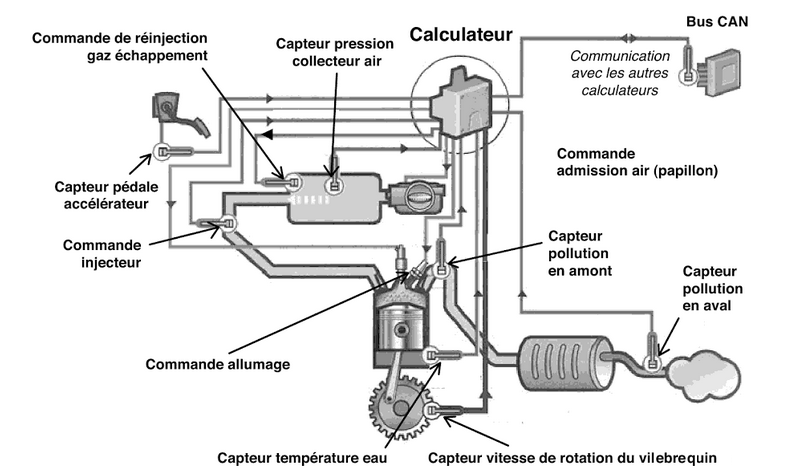
\includegraphics[width=\linewidth]{../Images/ControleCommande.png}
    \caption{Car's control command}
    \end{figure}
    \begin{itemize}
        \item Many tiny computers specialized for specifics tasks : ABS, motor optimization, lighting, climatisation, wheel pressure optimization, 
              mixing fuel/air, battery optimization, and so on.
        \item Computation must be terminated in constraint times;
        \item Lot of parameters are interdependants (external air temperature, wheel pressure, optimal speed and oil consommation)
    \end{itemize}
    \end{multicols}
\end{frame}

\begin{frame}[fragile]{Parallel computing example (1)}
    \framesubtitle{Control command (continuation)}
    \small
    \begin{multicols}{2}
        \begin{figure}[h]      
            
\includegraphics[width=\linewidth]{../Images/NuclearPlantSimpson.png}
            \caption{None Control Command of a reactor}
        \end{figure}
    \begin{itemize}
        \item Another control command : managing nuclear power reactors;
        \item High real time contraint algorithms;
        \item Lot of complex computations;
        \item One computing core isn't enough to satisty tiny real time constraints;
        \item \textcolor{blue}{\bf Solution} : Concurrency execution of interdependant tasks on many computing cores; 
    \end{itemize}
\end{multicols}
\end{frame}

\begin{frame}[fragile]{Parallel computation example (2)}
    \framesubtitle{Physical Simulation}
    \small
    \begin{multicols}{2}
        \begin{figure}[h]
            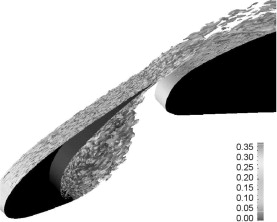
\includegraphics[width=\linewidth]{../Images/SlatWingTurb1.jpg}
            \caption{Turbulent noise generated by a plane's slate wing}
        \end{figure}

        \begin{itemize}
            \item Turbulence : very small phenomena (millimeter scale). Need a mesh with lof of tiny triangles;
            \item Typically, the mesh must contain five to ten billions of vertices with five unknowned variables for each vertex; 
            \item Minimum memory requirement : 7 To 
            \item Sequential computation time : 23 days to simulate ${\frac{1}{100}}^{e}$ seconds
        \end{itemize}
    \end{multicols}
\end{frame}

\begin{frame}[fragile]{Parallel computation example (3)}
  \framesubtitle{Artificial intelligence}
  \small
  \begin{multicols}{2}
        \begin{figure}[h]
            
\includegraphics[width=\linewidth]{../Images/HAL.png}
            \caption{A very famous artifical intelligence (HAL)}
        \end{figure}
        \begin{itemize}
        \item Deep learning used in AI to categorize pictures, automatic translations, Cancereous cells detection, automatic vehicles, and so.
        \item In sequential required more than one year to learn;
        \item with GPGPU, required about one month;
        \item \textcolor{blue}{March 2016} : Alphago wins versus world GO human champion (supervised learning);
        \item \textcolor{DarkGreen}{October 2017}: Alphago zero wins versus alphago at 100 games to zero (deep learning).
  \end{itemize}
  \end{multicols}
\end{frame}

\begin{frame}[fragile]{Parallel computation (4)}
  \framesubtitle{Picture treatment}
  \scriptsize
  \begin{figure}[h]
  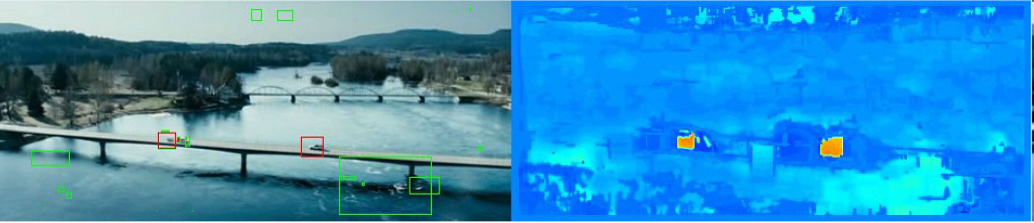
\includegraphics[width=\linewidth]{../Images/fluxvideo.png}
  \caption{Real time constraint treatment of a video with 30 frames/s (resolution 1920 $\times$ 1080 pixels)}
  \end{figure}

  \begin{itemize}
  \item Needed for optical captors for navigation of autonomous vehicules, for super-resolution picture issued from low resolution video, and so on.
  \item Lot of computations needed (PDE equation to solve);
  \item Must use GPGPU and parallel algorithms to have real time constraint;
  \end{itemize}
\end{frame}

\begin{frame}[fragile]{Top 10 of supercomputers (June 2020)}
  \small
  \begin{center}
  \begin{tabular}{|>{\columncolor{cyan!25}\bfseries}c|c|c|c|>{\columncolor{yellow!50}}c|c|}\hline
    \rowcolor{green!25} Name & Core & Perf. (TFlops) & Constructor      & Country  & Power (kW) \\ \hline\hline
    Fugaku            & 7 299 072 & 415 530 & Fujitsu    & Japan & 28 335 \\ \hline
    Summit            & 2 414 592 & 148 600 & IBM        & USA   & 10 096 \\ \hline
    Sierra            & 1 572 480 & 94  640 & IBM/NVidia & USA   &  7 438 \\ \hline
    Sunway TaihuLight & 10 649 600 & 93 014 & NRCPC      & China & 15 371 \\ \hline
    Tianhe-2A         &  4 981 760 & 61 444 & NUDT       & China & 18 482 \\ \hline
    HPC5              &    669 760 & 35 450 & Dell EMC   & Italy &  2 252 \\ \hline
    Selene            &    277 760 & 27 580 & Nvidia     & USA   &  1 344 \\ \hline
    Frontera          &    448 448 & 23 516 & Dell EMC   & USA   &  ?     \\ \hline
    Marconi-100       &    347 776 & 21 640 & IBM        & Italy &  1 476 \\ \hline
    Frontier          &    591 872 &  1 102 & HPE        & USA   & 21 000 \\ \hline
  \end{tabular}
  \end{center}
  \textbf{\textcolor{blue}{Remarque}} : Nowaday, we look for Flops/Watt performances
\end{frame}

\section{Classification of parallel architectures}

\subsection{Shared memory}

\begin{frame}[fragile]{shared memory architecture}
  \scriptsize

 \begin{multicols}{2}
  \begin{figure}[ht]
    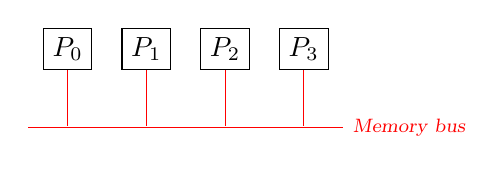
\begin{tikzpicture}
      \foreach \x\n in {-2/$P_{0}$,-1/$P_{1}$,0/$P_{2}$,1/$P_{3}$} {        
        \node[draw] (P\x) at (\x,1) {\n};
        \node[anchor=center,inner sep=0pt] (M\x) at (\x,0) {};
     }
      \draw[color=red] (-2.5,0) -- (1.5,0) node[anchor=west] {\scriptsize \textcolor{red}{\sl Memory bus}};
      \foreach \x in {-2,-1,0,1} {        
        \draw[color=red] (P\x) -- (M\x);
      }
    \end{tikzpicture}
    \caption{\scriptsize Simplified scheme of memory shared parallel architecture}
  \end{figure}

  Many computing cores shared the same main memory
  
  \begin{exampleblock}{Exemples}
    \begin{itemize}
    \item The recent muti-cores processors;
    \item The graphic cards with 3D acceleration;
    \item The phones, pad, etc.
    \end{itemize}
  \end{exampleblock}

  \begin{alertblock}{Memory access problem}
    \begin{itemize}
    \item Optimization of memory access.
    \item Simultaneous read/write accesses at same memory location.
    \end{itemize}
  \end{alertblock}
  
  \end{multicols}
\end{frame}

\begin{frame}[fragile]{Memory access}

  \begin{figure}[ht]
    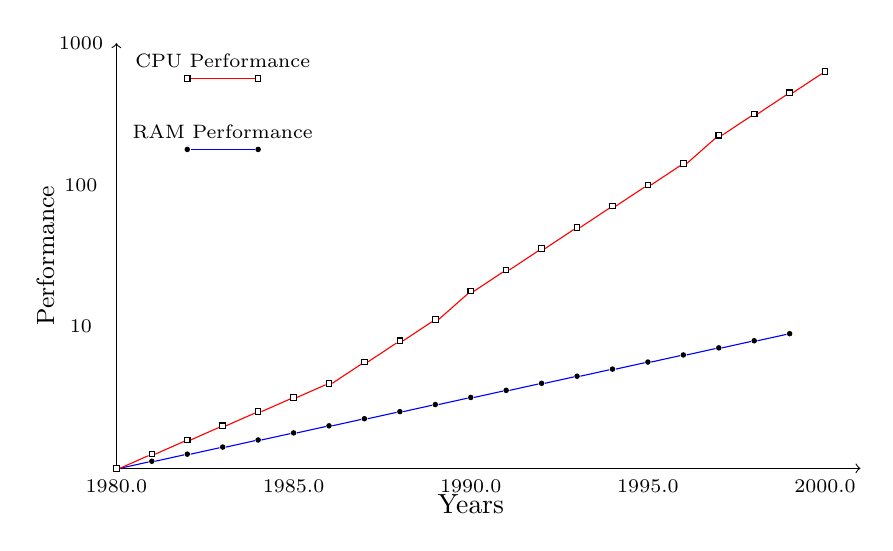
\begin{tikzpicture}[scale=0.9]
      \draw[color=black,->](0,0) -- (10.5,0);
      \draw[color=black,->](0,0) -- (0,6);
      \node at (5,-0.5) {Years};
      \foreach \a in {0,5,...,20} {
        \tikzmath{\an=1980+\a;}
        \node at (0.5*\a,-0.25) {\scriptsize \an};
      }
      \node[rotate=90] at (-1.,3) {\small Performance};
      \node at (-0.5,2) {\scriptsize 10};
      \node at (-0.5,4) {\scriptsize 100};
      \node at (-0.5,6) {\scriptsize 1000};
      \node[circle,fill=black,minimum size=2pt,inner sep=0pt] (M0) at (0.,0.) {};
      \foreach \i in {1,2,...,19} {
        \def\x{0.5*\i}
        \def\p{0.1*\i}
         \tikzmath{\im = \i-1;}
        \node[circle,fill=black,minimum size=2pt,inner sep=0pt] (M\i) at (\x,\p) {};
        \draw[color=blue] (M\im) -- (M\i);        
      }
      \node[fill=white,draw, minimum size=2pt, inner sep=1pt] (P0) at (0,0) {};
      \foreach \a/\y in {1/0.2,2/0.4,3/0.6,4/0.8,5/1.0,6/1.2,7/1.5,8/1.8,9/2.1,10/2.5,11/2.8,12/3.1,13/3.4,14/3.7,15/4.0,16/4.3,17/4.7, 18/5.0, 19/5.3, 20/5.6} {
      \tikzmath{\am=\a-1;}
      \node[fill=white,draw, minimum size=2pt, inner sep=1pt] (P\a) at (0.5*\a,\y) {};
      \draw[color=red] (P\am) -- (P\a);
      }
      \node[fill=white,draw, minimum size=2pt, inner sep=1pt](L1) at (1,5.5){};
      \node[fill=white,draw, minimum size=2pt, inner sep=1pt] (L2) at (2,5.5) {};
      \node at (1.5,5.75) {\scriptsize CPU Performance};
      \draw[color=red]  (L1) -- (L2); 

      \node[circle, fill=black, minimum size=2pt, inner sep=0pt] (L3) at (1,4.5){};
      \node[circle, fill=black, minimum size=2pt, inner sep=0pt] (L4) at (2,4.5) {};
      \node at (1.5,4.75) {\scriptsize RAM Performance};
      \draw[color=blue]  (L3) -- (L4); 

    \end{tikzpicture}
  \end{figure}
\end{frame}

\begin{frame}[fragile]{Latency memory example (Haswell architecture)}
  \scriptsize

  \begin{center}
  \begin{tabular}{|>{\columncolor{orange!25}\bfseries}c|c|c|c|}\hline
    \rowcolor{cyan!25}Level & Size & Latency (cycles) & Physical location \\ \hline\hline
    L1 Cache & 16/16 ko & 4 & In each core \\ \hline
    L2 Cache & 256   ko & 12& Shared by two cores \\ \hline
    L3 Cache & 12    Mo & 21& Shared by all cores \\ \hline
    Ram      & 32    Go & 117 & SRAM on mother board \\ \hline
    Swap     & 100+  Go & 10 000 & Hard disk or SSD \\ \hline
  \end{tabular}
\end{center}

\begin{alertblock}{Conclusion}
\begin{itemize}
    \item Memory is more and more slower comparing to the instruction execution of the processor; 
    \item It's worst with multicore architecture !
\end{itemize}
\end{alertblock}

\end{frame}

\begin{frame}[fragile]{How works a RAM ?}

    \begin{figure}[ht]
        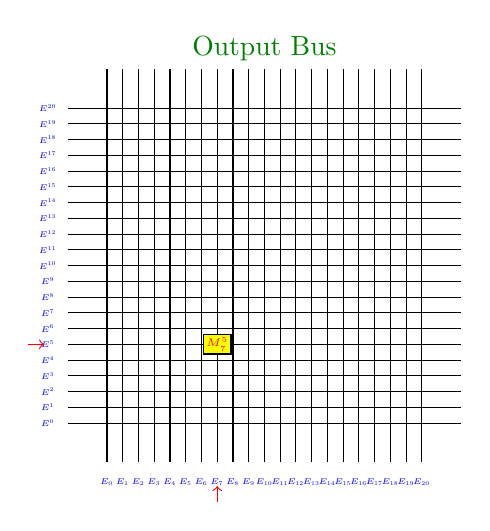
\begin{tikzpicture}
        \foreach \i in {0,1,2,...,20}
        {
            \node at (0.2*\i,-0.75) {\fontsize{3pt}{3.6pt}\selectfont\color{blue} $E_{\i}$};
            \node at (-0.75, 0.2*\i) {\fontsize{3pt}{3.6pt}\selectfont\color{blue} $E^{\i}$};
            \draw  (0.2*\i,-0.5) -- (0.2*\i,4.5);
            \draw (-0.5,0.2*\i) -- (4.5,0.2*\i) ;
        }
        \draw[->,red] (-1.0, 1.0) -- (-0.8, 1.0);
        \draw[->,red] ( 1.4,-1.0) -- ( 1.4,-0.8);
        \node[fill=Yellow,draw,inner sep=1pt] at (1.4,1.0) {\fontsize{4pt}{4pt}\selectfont\color{red}\bf$M_{7}^{5}$};
        \node at (2,4.75) {\textcolor{DarkGreen}{Output Bus}};
    \end{tikzpicture}
\end{figure}
\end{frame}

\begin{frame}{Interleaved rams}
    \small
    \begin{center}
        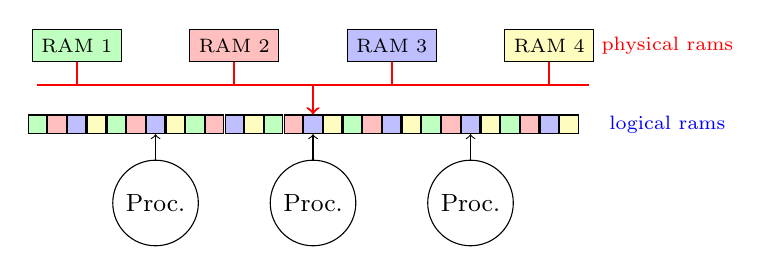
\begin{tikzpicture}
           \node[fill=green!25!white,draw] at (-3,0) (R1) {\scriptsize RAM 1}; 
           \node[fill=red!25!white,draw] at (-1,0) (R2) {\scriptsize RAM 2}; 
           \node[fill=blue!25!white,draw] at (+1,0) (R3) {\scriptsize RAM 3}; 
           \node[fill=yellow!25!white,draw] at (+3,0) (R4) {\scriptsize RAM 4};
           \node at (4.5,0) {\scriptsize \textcolor{red}{physical rams}};
           \foreach \x in {-3.5,-2.5,-1.5,...,2.5}
           {
            \node[fill=green!25!white,draw,minimum size=0.25] at (\x,-1) {};
            \node[fill=red!25!white,draw,minimum size=0.25] at (\x+0.25,-1) {};
            \node[fill=blue!25!white,draw,minimum size=0.25] at (\x+0.5,-1) {};
            \node[fill=yellow!25!white,draw,minimum size=0.25] at (\x+0.75,-1) {};
           }
           \draw[thick, red] (-3.5,-0.5) -- (3.5,-0.5);
           \draw[thick, red] (R1) -- (-3,-0.5);
           \draw[thick, red] (R2) -- (-1,-0.5);
           \draw[thick, red] (R3) -- (+1,-0.5);
           \draw[thick, red] (R4) -- (+3,-0.5);
           \draw[thick, red, ->] (0,-0.5) -- (0,-0.875);
           \node at (4.5,-1) {\scriptsize \textcolor{blue}{logical rams}};

           \node[circle, draw] at (-2,-2) (P1) {\small Proc.};
           \node[circle, draw] at ( 0,-2) (P2) {\small Proc.};
           \node[circle, draw] at ( 2,-2) (P3) {\small Proc.};
           \draw[->] (P1) -> (-2,-1.125);
           \draw[->] (P2) -> ( 0,-1.125);
           \draw[->] (P3) -> (+2,-1.125);
        \end{tikzpicture}
    \end{center}
    \begin{block}{\small Interleaved memory}
        \begin{itemize}
            \item Many physical memory units interleaved by the memory bus;
            \item Number of physical memory units $\equiv$ number of ways;
            \item Number of contiguous bytes in a unique physical memory $\equiv$ width of way;
            \item \alert{Quadratic cost to build relative to number of memory units} !
        \end{itemize}
       \end{block}
\end{frame}

\begin{frame}[fragile]{Interleaved memory access}

    \begin{block}{\small Classic memory access}
    {\scriptsize
    \begin{center}
    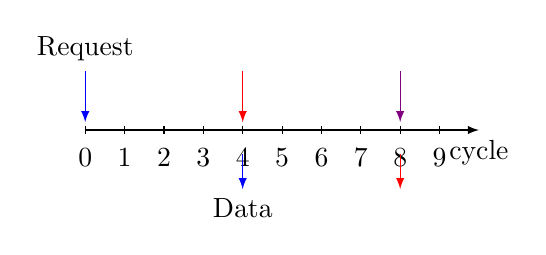
\begin{tikzpicture}[scale=0.5]
    \draw[->,>=latex] (0,0) -- (10,0) node[below]{cycle};
    \foreach \x in {0,1,...,9} {
      \draw (\x,1mm) -- (\x,-1mm) node[below] {$\x\strut$};
    }
    \draw[->,>=latex,blue] (0,1.5cm) node[above,black] {Request} -- (0,2mm);
    \draw[->,>=latex,red] (4,1.5cm) -- (4,2mm);
    \draw[->,>=latex,violet] (8,1.5cm) -- (8,2mm);
    
    \draw[->,>=latex,blue] (4,-4ex) -- (4,-1.5cm) node[below,black]{Data};
    \draw[->,>=latex,red] (8,-4ex) -- (8,-1.5cm);
    \end{tikzpicture}
    \end{center}
    }
    \end{block}
    
    \begin{block}{\small four ways interleaved memory access}
    {\scriptsize
    \begin{center}
    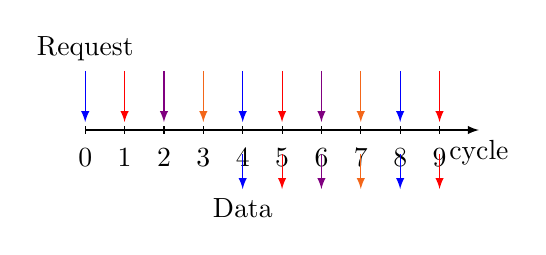
\begin{tikzpicture}[scale=0.5]
    \draw[->,>=latex] (0,0) -- (10,0) node[below]{cycle};
    \foreach \x in {0,1,...,9} {
      \draw (\x,1mm) -- (\x,-1mm) node[below] {$\x\strut$};
    }
    \draw[->,>=latex,blue] (0,1.5cm) node[above,black] {Request} -- (0,2mm);
    \foreach \x/\col in {1/red,2/violet,3/ocre,4/blue,5/red,6/violet,7/ocre,8/blue,9/red}{
      \draw[->,>=latex,\col] (\x,1.5cm) -- (\x,2mm);
    }
    \draw[->,>=latex,blue] (4,-4ex) -- (4,-1.5cm) node[below,black] {Data};
    \foreach \x/\col in {5/red,6/violet,7/ocre,8/blue,9/red}{
      \draw[->,>=latex,\col] (\x,-4ex) -- (\x,-1.5cm);
    }
    \end{tikzpicture}
    \end{center}
    }
    \end{block}
\end{frame}
    

\begin{frame}[fragile]{Cache memory}
    \begin{block}{Consequences of grid architecture of RAMS}
        Bigger is a memory, bigger is her grid, slower is the read and write access.
    \end{block}

    \begin{exampleblock}{Cache memory}
        \begin{itemize}
            \item Fast small memory unit where one store temporary data;
            \item When multiple access to a same variable \alert{in a short time}, speedup the read or write access;
            \item Cache memory managed by the CPU (but cache memory for GPU can be managed by the programmer);
            \item \textbf{Consequence} : To optimize his program, the programmer must know the strategies used by the CPU.
        \end{itemize}
    \end{exampleblock}
\end{frame}


\begin{frame}[fragile]{Cache memory}
    \begin{block}{CPU Strategy}
        \begin{itemize}
            \item \textbf{Cache line} : store contiguous memory variables in cache (64 bytes on intel processor);
            \item \textbf{Associative memory cache} : Each cache memory address mapped on fixed RAM address (with a modulo).
        \end{itemize}
    \end{block}

    \begin{alertblock}{Consequences}
        \begin{itemize}
            \item Better to have contiguous access in memory;
            \item Better to use as soon as possible data stored in cache;
            \item \alert{Spatial and time localisation of data}.
        \end{itemize}
    \end{alertblock}
\end{frame}



\begin{frame}[fragile]{memory organization on multi-processor computer}
    \scriptsize
    \begin{center}
    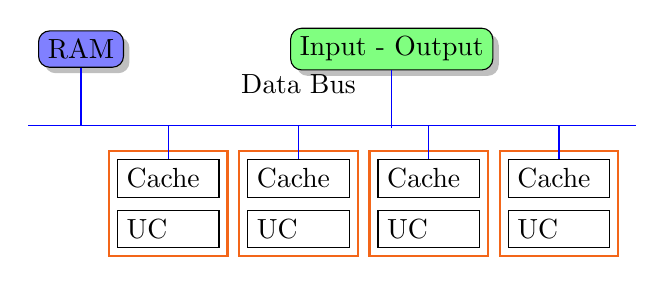
\begin{tikzpicture}
    \node[rounded corners, drop shadow,draw,fill=blue!50!white,text height=1.5ex] (M) {RAM};
    \node[rounded corners, drop shadow,draw,fill=green!50!white, right= 6em of M.east, text height=1.5ex] (E) {Input - Output};
    \node[below=4ex of M.south] (B) {};
    \node[below=4ex of E.south] (Be) {};
    \node[below=4ex of M.south west] (B0) {};
    \foreach \x/\n in {1/B0,2/B1,3/B2,4/B3} {
      \node[right=4em of \n.east] (B\x) {};
      \node[below=2ex of B\x.south,draw,text width=3em] (C\x) {Cache};
      \node[below=1ex of C\x.south,draw,text width=3em] (P\x) {UC};
      \draw[ocre,thick] ($(C\x.north west)+(-0.1,0.1)$) rectangle ($(P\x.south east)+(0.1,-0.1)$);
      \draw[blue] (B\x.center) -- (C\x);
    }
    \node[right=4ex of B4.east] (B5) {};
    \draw[blue] (B0.west) -- (B5.east);
    \draw[blue] (M) -- (B.center);
    \draw[blue] (E) -- (Be.center);
    \node[above= 1 ex of B2.north] {Data Bus};
    \end{tikzpicture}
    \end{center}
    
    Data coherence between memory caches :
    
    {\scriptsize
    \begin{itemize}
    \item An unique cache contains the datum : value is valid, none synchronization needed;
    \item Datum shared with another memory caches : At each access, verify if the datum is modified by another core and write as invalid when modifiying his value;
    \item Modify the value in the cache : value now not valid in RAM : update the value in RAM if another core reads the value;
    \item Value is invalid for cache. The next read of this value must access of the value in RAM.
    \end{itemize}
    }
    
    \end{frame}

    \begin{frame}[fragile]{Many cores cache organization}

        \scriptsize
        \begin{center}
        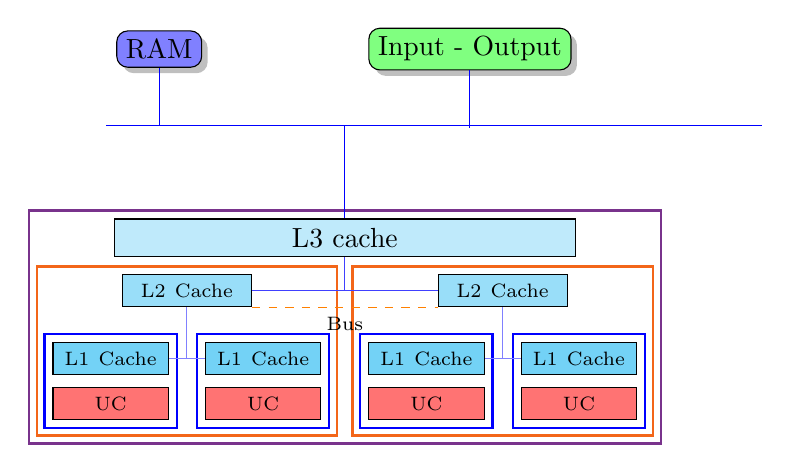
\begin{tikzpicture}
        \node[rounded corners, drop shadow,draw,fill=blue!50!white,text height=1.5ex] (M) {RAM};
        \node[rounded corners, drop shadow,draw,fill=green!50!white, right= 6em of M.east, text height=1.5ex] (E) {Input - Output};
        \node[below=4ex of M.south] (B) {};
        \node[below=4ex of E.south] (Be) {};
        \node[below=4ex of M.south west] (B0) {};
        \node[right=6em of B.east] (B1) {};
        \node[right=14em of B1.east] (Br) {};
        \node[below=7ex of B1.south,text width = 16em,fill=cyan!25,draw,text centered] (L3) {L3 cache};
        \node[below=2ex of L3.south] (BL3) {};
        \node[left=3em of BL3.west,draw,text width = 4em,fill=cyan!40,text centered] (L21) {\scriptsize L2 Cache};
        \node[right=3em of BL3.east,draw,text width = 4em,fill=cyan!40, text centered] (L22) {\scriptsize L2 Cache};
        
        \node[below=1.5em of L21.south] (BL21) {};
        \node[left=0.3em of BL21.west,draw,text width = 3.5em,fill=cyan!55, text centered] (L111) {\scriptsize L1 Cache};
        \node[below=1ex of L111.south,draw,text width = 3.5em,fill=red!55, text centered] (U111) {\scriptsize UC};
        \draw[blue,thick] ($(U111.south west)+(-0.1,-0.1)$) rectangle ($(L111.north east)+(0.1,0.1)$);
        \node[right=0.3em of BL21.east,draw,text width = 3.5em,fill=cyan!55, text centered] (L112) {\scriptsize L1 Cache};
        \node[below=1ex of L112.south,draw,text width = 3.5em,fill=red!55, text centered] (U112) {\scriptsize UC};
        \draw[blue,thick] ($(U112.south west)+(-0.1,-0.1)$) rectangle ($(L112.north east)+(0.1,0.1)$);
        
        \node[below=1.5em of L22.south] (BL22) {};
        \node[left=0.3em of BL22.west,draw,text width = 3.5em,fill=cyan!55, text centered] (L121) {\scriptsize L1 Cache};
        \node[below=1ex of L121.south,draw,text width = 3.5em,fill=red!55, text centered] (U121) {\scriptsize UC};
        \draw[blue,thick] ($(U121.south west)+(-0.1,-0.1)$) rectangle ($(L121.north east)+(0.1,0.1)$);
        \node[right=0.3em of BL22.east,draw,text width = 3.5em,fill=cyan!55, text centered] (L122) {\scriptsize L1 Cache};
        \node[below=1ex of L122.south,draw,text width = 3.5em,fill=red!55, text centered] (U122) {\scriptsize UC};
        \draw[blue,thick] ($(U122.south west)+(-0.1,-0.1)$) rectangle ($(L122.north east)+(0.1,0.1)$);
        
        \draw[ocre,thick] ($(U111.south west)+(-0.2,-0.2)$) rectangle ($(L21.north -| L112.east)+(0.2,0.1)$);
        \draw[ocre,thick] ($(U121.south west)+(-0.2,-0.2)$) rectangle ($(L22.north -| L122.east)+(0.2,0.1)$);
        
        \draw[ocre!50!blue,thick] ($(U111.south west)+(-0.3,-0.3)$) rectangle ($(L3.north -| L122.east)+(0.3,0.1)$);
        
        \draw[blue] (B0.west) -- (Br.east);
        \draw[blue] (M) -- (B.center);
        \draw[blue] (E) -- (Be.center);
        \draw[blue] (B1.center) -- (L3);
        \draw[blue!75] (L3) -- (BL3.center);
        \draw[blue!75] (BL3.center) -- (L21);
        \draw[blue!75] (BL3.center) -- (L22);
        \draw[blue!50] (L21) -- (BL21.center);
        \draw[blue!50] (BL21.center) -- (L111);
        \draw[blue!50] (BL21.center) -- (L112);
        
        \draw[blue!50] (L22) -- (BL22.center);
        \draw[blue!50] (BL22.center) -- (L121);
        \draw[blue!50] (BL22.center) -- (L122);
        \draw[orange,dashed] (L21.south east) -- node[below] {\scriptsize \textcolor{black}{Bus}} (L22.south west);
        \end{tikzpicture}
        \end{center}
        
        Same issue with cache coherency, but need too coherence of data between cache levels. Complexity raises with the number of 
        cache levels.
        
        \end{frame}


\begin{frame}[fragile]{Tools for shared memory computation}
\small
Many tools can be used to use many "threads" and the synchronization in memory. The most used are :

\begin{itemize}
  \item OpenMP : Compilation directives and small C API (\mintinline{C++}{#pragma});
  \item Standard library in C++ (threads, asynchronous functions);
  \item TBB (Threading Building Block library, Intel) : Open source library from Intel
  \end{itemize}
 
But memory conflict access must be cared for the programmer :
\begin{itemize}
    \item When a thread writes a datum and some other threads read simultaneously the same datum;
    \item When some thread writes at the same datum;
    \item Doesn't rely on the instruction order in the program ! (out-of-order optimization by compiler and processor).
\end{itemize}
\end{frame}

\subsection{Distributed memory}

\begin{frame}[fragile]{Distributed memory}
    \scriptsize
    \begin{center}
    {
    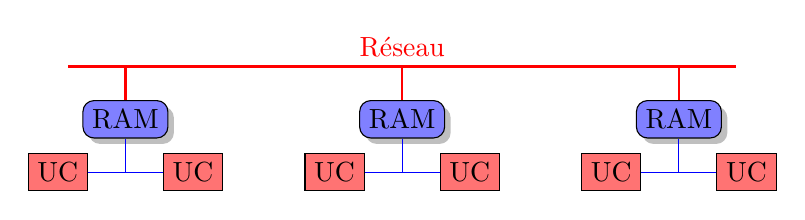
\begin{tikzpicture}[scale=0.5]
    \node[draw,fill=blue!50!white, drop shadow, rounded corners] (Ram1) {RAM};
    \node[below=2ex of Ram1.south] (B1) {};
    \node[left=1em of B1.west,draw,fill=red!55] (U1) {UC};
    \node[right=1em of B1.east,draw,fill=red!55] (U2) {UC};
    \draw[blue] (Ram1) -- (B1.center);
    \draw[blue] (B1.center) -- (U1);
    \draw[blue] (B1.center) -- (U2);
    
    \node[draw,fill=blue!50!white, drop shadow, rounded corners,left=10em of Ram1.east] (Ram2) {RAM};
    \node[below=2ex of Ram2.south] (B2) {};
    \node[left=1em of B2.west,draw,fill=red!55] (U3) {UC};
    \node[right=1em of B2.east,draw,fill=red!55] (U4) {UC};
    \draw[blue] (Ram2) -- (B2.center);
    \draw[blue] (B2.center) -- (U3);
    \draw[blue] (B2.center) -- (U4);
    
    \node[draw,fill=blue!50!white, drop shadow, rounded corners,left=10em of Ram2.east] (Ram3) {RAM};
    \node[below=2ex of Ram3.south] (B3) {};
    \node[left=1em of B3.west,draw,fill=red!55] (U5) {UC};
    \node[right=1em of B3.east,draw,fill=red!55] (U6) {UC};
    \draw[blue] (Ram3) -- (B3.center);
    \draw[blue] (B3.center) -- (U5);
    \draw[blue] (B3.center) -- (U6);
    
    \node[above=2ex of Ram1.north] (R1) {};
    \node[above=2ex of Ram2.north] (R2) {};
    \node[above=2ex of Ram3.north] (R3) {};
    \node[right=1em of R1.east] (R0){};
    \node[left=1em of R3.west] (R4) {};
    \draw[thick,red] (R0.east) -- (R1.center) -- (R2.center) node[above] {Réseau}-- (R3.center) -- (R4.west);
    \draw[thick,red] (Ram1) -- (R1.center);
    \draw[thick,red] (Ram2) -- (R2.center);
    \draw[thick,red] (Ram3) -- (R3.center);
    \end{tikzpicture}
    }
    \end{center}
    
    \begin{itemize}
      \item Each computing unit can read/write on local ram : the set containing the computing unit and the ram is called \textbf{Computing node};
      \item The data are exchanged between computing nodes through a specialized bus or specific ethernet link;
      \item On ethernet link, it's the responsability of the programmer to exchange explicitly the data between computing nodes;
      \item Need specifics efficiency algorithms and a library;
      \item Possible to compute on many thousands of computing cores;
      \item Only limited by electricity consumption (linear cost);
     \end{itemize}    
    \end{frame}

\begin{frame}[fragile]{Distributed parallelism context}
    \small
    All libraries managing the distributed parallelims computation provide similars functionnalities.

    \begin{block}{\small Running an distributed parallel application}
        \begin{itemize}
            \item An application is provided to the user to run his application(s) on a wanted number \texttt{nbp} of computing nodes (given when running the application);
            \item The computing nodes where the application(s) is launched is defined by default or in a file provided by the user;
            \item The default output for all processes are the terminal output from which was launched the application;
            \item A communicator (defining a set of processes) is defined by default including all launched processes (\verb@MPI_COMM_WORLD@);
            \item The application gives an unique number for each process in a communicator (numbering from zero to \texttt{nbp}-1);
            \item All processes terminates the program at the same time;
        \end{itemize}
    \end{block}
\end{frame}

\begin{frame}[fragile]{Managing the context in your program}
    \small
    \begin{itemize}
        \item Call initialization of parallel context before using other function in the library (\verb@MPI_Init@);
        \item Get the number of processes contained by the communicator (\verb@MPI_Comm_size@);
        \item Read the rank of the process inside the communicator (\verb@MPI_Comm_rank@);
        \item After calling the last library function, call the termination of parallel context to synchronize processes (\verb@MPI_Finalize@, if not done, crash your program).
    \end{itemize}

\begin{minted}{C++}
#include <mpi.h>
int main(int nargs, char const* argv[])
{
    MPI_Comm commGlob;
    int nbp, rank;
    MPI_Init(&nargs, &argv);// Initialization of the parallel context
    MPI_Comm_dup(MPI_COMM_WORLD, &commGlob);// Copy global communicator in own communicator;
    MPI_Comm_size(commGlob, &nbp);// Get the number of processes launched by the used;
    MPI_Comm_rank(commGlob, &rank);// Get the rank of the process in the communicator commGlob.
    ...
    MPI_Finalize();// Terminates the parallel context
}
\end{minted}

\end{frame}

\begin{frame}[fragile]{Point to point data echange}
    \scriptsize
    A process send some data in a message to another process which receives this message.
    \begin{multicols}{2}
    \begin{block}{\small Constitution of a data message to send}
        \begin{itemize}
            \item The communicator used to send the data;
            \item The memory address of the contiguous data to send;
            \item The number of data to send;
            \item The type of the data (integer, real, user def type, and so.);
            \item The rank of destination process;
            \item A tag number to identify the message
        \end{itemize}
    \end{block}
    \begin{block}{\small Constitution of a data message to receive}
        \begin{itemize}
            \item The communicator used to receive the data;
            \item A memory address of a buffer where store the received data;
            \item the number of data to receive;
            \item The type of the data (integer, real, user def type, and so.)
            \item The rank of the sender process (can be any process);
            \item A tag number to identify the message (can be any tag if needed)
            \item Status of the message (receive status, error, sender, tag);
        \end{itemize}
    \end{block}
\end{multicols}

\begin{minted}{C++}
    if (rank == 0) {
        double vecteur[5] = { 1., 3., 5., 7., 22. };
        MPI_Send(vecteurs, 5, MPI_DOUBLE, 1, 101, commGlob);    }
    else if (rank==1) {
        MPI_Status status;    double vecteurs[5];
        MPI_Recv(vecteurs, 5, MPI_DOUBLE, 0, 101, commGlob, &status);    }
\end{minted}

\end{frame}

\begin{frame}[fragile]{Interlocking}
    \scriptsize
    \begin{block}{Definition}
        \begin{itemize}
            \item Interlocking is a situation where many processes are waiting each other for a infinite time to complete their messages;
            \item By example, process one wait to receive a message from 0 and 0 wait to receive a message from 1;
            \item Or process zero sends a message to 1 and process one wait a message from 0 but with wrong tag !
            \item Sometimes, interlocking can be very hard to find !
            \item \textbf{Rule of thumb} : Be careful for each send to have a corresponding receive with right tag and expeditor.
        \end{itemize}
    \end{block}

\begin{minted}{C++}
if (rank==0)
{
    MPI_Recv(rcvbuf, count, MPI_DOUBLE, 1, 101, commGlob, &status);
    MPI_Send(sndbuf, count, MPI_DOUBLE, 1, 102, commGlob);
}
else if (rank==1)
{
    MPI_Recv(rcvbuf, count, MPI_DOUBLE, 0, 102, commGlob, &status);
    MPI_Send(sndbuf, count, MPI_DOUBLE, 0, 101, commGlob);
}
\end{minted}
\end{frame}

\begin{frame}[fragile]{Interlocking (more complicated cases)}

    \begin{minted}{C++}
    MPI_Comm_rank(comm, &myRank ) ;
    if (myRank == 0 ) 
    {
        MPI_Ssend( sendbuf1, count, MPI_INT, 2, tag, comm);
        MPI_Recv( recvbuf1, count, MPI_INT, 2, tag, comm, &status);
    } 
    else if ( myRank == 1 ) 
    {
        MPI_Ssend( sendbuf2, count, MPI_INT, 2, tag, comm);
    }
    else if ( myRank == 2 ) 
    {
        MPI_Recv( recvbuf1, count, MPI_INT, MPI_ANY_SOURCE, tag, comm,
                 &status );
        MPI_Ssend( sendbuf2, count, MPI_INT, 0, tag, comm);
        MPI_Recv( recvbuf2, count, MPI_INT, MPI_ANY_SOURCE, tag, comm,
                 &status );
    }    
    \end{minted}
    \end{frame}
    

\begin{frame}[fragile]{Blocking and non blocking message}
    \scriptsize
    \begin{block}{Definition}
        \begin{itemize}
            \item Blocking message : Wait the complete reception of the message before returning from the function;
            \item Non blocking message : Post the message to send or receive and return from the function immediatly ! 
            \item The status of non blocking message is update in a request struct. (not yet send/recv, sending/receiving or sended/received)
            \item Allows to test or wait for the message to be completed. 
        \end{itemize}
    \end{block}

    \begin{exampleblock}{When use no blocking message ?}
        \begin{itemize}
            \item When one can compute using other data during messages exchanges to hide message exchange cost;
            \item To simplify algorithms to ensure none interlocking situations.
        \end{itemize}
    \end{exampleblock}

\end{frame}

\begin{frame}[fragile]{Example using non blocking message}
    
    \begin{minted}{C++}
        MPI_Request req;
        if (rank == 0) 
        {
            double vecteur[5] = { 1., 3., 5., 7., 22. };
            MPI_Isend(vecteurs, 5, MPI_DOUBLE, 1, 101, commGlob, &req);
            // Some compute with other data can be executed here!
            MPI_Wait(req, MPI_STATUS_IGNORE);
        }
        else if (rank==1) 
        {
            MPI_Status status;    double vecteurs[5];
                MPI_Irecv(vecteurs, 5, MPI_DOUBLE, 0, 101, commGlob, &req);
            int flag = 0;
            do {
                // Do computation while message is not received on another data
                MPI_Test(&req, &flag, &status);
            } while(flag );
        }
        \end{minted}
\end{frame}

\begin{frame}[fragile]{A scheme to avoid interlocking situations}
    \scriptsize
    \begin{block}{The scheme for all processes}
        \begin{itemize}
        \item First do receptions in non blocking mode;
        \item Second, do send in blocking mode (or non blocking mode if you want to overlay message cost with computing)
        \item Third, synchronize yours receptions (waiting for completion or testing to overlay message cost with computing).
        \end{itemize}
    \end{block}
    \begin{minted}{C++}
        MPI_Request req; MPI_Status status;
        if (rank==0)
        {
            MPI_Irecv(rcvbuf, count, MPI_DOUBLE, 1, 101, commGlob, &req);
            MPI_Send(sndbuf, count, MPI_DOUBLE, 1, 102, commGlob);
            MPI_Wait(&req, &status);
        }
        else if (rank==1)
        {
            MPI_Irecv(rcvbuf, count, MPI_DOUBLE, 0, 102, commGlob, &req);
            MPI_Send(sndbuf, count, MPI_DOUBLE, 0, 101, commGlob);
            MPI_Wait(&req, &status);
        }
        \end{minted}
\end{frame}


\begin{frame}[fragile]{Bufferized or non bufferized messages}

    \begin{block}{Bufferized messages}
        \begin{itemize}
            \item A non blocking send is copied in a buffer before to be sended;
            \item $\Rightarrow$ \textcolor{DarkGreen}{After calling a non blocking send, the user can modify the sended data without
                  changing the values to send};
            \item It's the default behavior when we send a message
            \item But the copy of the data in a buffer has a memory and cpu cost !
            \item We can to call send functions which doesn't copy the data in a buffer;
            \item \alert{It's the responsability of the user to avoid to change data before the synchronization of the message !}
        \end{itemize}
    \end{block}
\end{frame}

\begin{frame}[fragile]{Example of non bufferized messages}
    \begin{multicols}{2}
\begin{minted}{c++}
std::vector<double> tab{3.,5.,7.,11.};
// Blocking non bufferized send
MPI_Ssend(tab.data(), tab.size(), 
          MPI_DOUBLE, 1, 104, commGlob);
// OK, tab is sended when we 
//     modify the buffer
tab[3] = 13.;
\end{minted}
\textcolor{DarkGreen}{Right example}
\begin{minted}{c++}
std::vector<double> tab{3.,5.,7.,11.};
// Non blocking non bufferized send
MPI_Issend(tab.data(), tab.size(), 
           MPI_DOUBLE, 1, 104, commGlob,&request);
MPI_Wait(&request, &status);
// OK, tab is sended when we 
//     modify the buffer
tab[3] = 13.;
\end{minted}
\textcolor{DarkGreen}{Right example}
    
\columnbreak
\begin{minted}{c++}
std::vector<double> tab{3.,5.,7.,11.};
// Non blocking non bufferized send
MPI_Issend(tab.data(), tab.size(), 
           MPI_DOUBLE, 1, 104, commGlob,&request);
// ERROR, we modify the buffer before
//        than the tab is sended !
tab[3] = 13.;
\end{minted}
\textcolor{red}{Wrong example}
\end{multicols}
\end{frame}

\begin{frame}[fragile]{Collective messages}
\scriptsize
\begin{exampleblock}{\scriptsize What is the collective communication}
    \begin{itemize}
        \item Broadcast data from one process to all processes;
        \item Scatter data from one process to all processes;
        \item Gather data from all processes to one process;
        \item Reduce data (with arithmetic operation) from all processes to one/all processes
        \item Scan data (with arithmetic operation) from all processes to all processes
        \item All to all broadcast/scatter data
    \end{itemize}
\end{exampleblock}

\begin{alertblock}{\scriptsize Why collective communication}
\begin{itemize}
    \item Point to point communication is enough for all algorithms !
    \item But, for some parallel operations (broadcasting, reduction, scattering), the optimal algorithm depends on net topology;
    \item Distributed parallel libraries provides collective communication which are optimized for all net topology;
\end{itemize}
\end{alertblock}
\end{frame}

\begin{frame}[fragile]{Distributed parallel rules}

    \begin{itemize}
        \item Ethernet data exchange is very slow comparing to memory access : \textcolor{blue}{limit as possible the data exchanges};
        \item To hide data exchange cost, it's better to compute some values during the exchange of data : \textcolor{blue}{prefer to use non blocking message exchange}
        \item Each message has an initial cost : \textcolor{blue}{prefer to regroup data in a temporary buffer if needed};
        \item All processes quit the program at the same time : \textcolor{blue}{Try to balance the computing load of computing nodes};
    \end{itemize}
\end{frame}

    \begin{frame}[fragile]{Disponible tools}

        \begin{itemize}
            \item Program ethernet layers (for specialists only !);
            \item Use dedicaced library (MPI, PVM, ...)
        \end{itemize}

        In all cases, data exchanges messages must call explicitly, calling functions provided by the library;

        Better to think his software in parallel at the beginning of the project.
    \end{frame}

\end{document}
